%%%%%%%%%%%%%%%%%%%%%%%%%%%%%%%%%%%%%%%%%
% Apéndice: Evidencias técnicas         %
%%%%%%%%%%%%%%%%%%%%%%%%%%%%%%%%%%%%%%%%%

\chapter{Evidencias técnicas}
\label{ap:evidencias-tecnicas}


%%%%%%%%%%%%%%%%%%%%%%%%%%%%%%%%%%%%%%%%%
% Arquitectura detallada                %
%%%%%%%%%%%%%%%%%%%%%%%%%%%%%%%%%%%%%%%%%

\section{Arquitectura detallada}
\label{ap:arquitectura-detallada}

La figura~\ref{fig:arquitectura-detallada} amplía la representación
simplificada presentada en el capítulo~5 e incorpora los principales
componentes internos del frontend y del backend, el procesamiento asíncrono
mediante Spring Batch, las fuentes de datos y los elementos de
infraestructura utilizados durante el despliegue.

\begin{figure}[H]
  \centering
  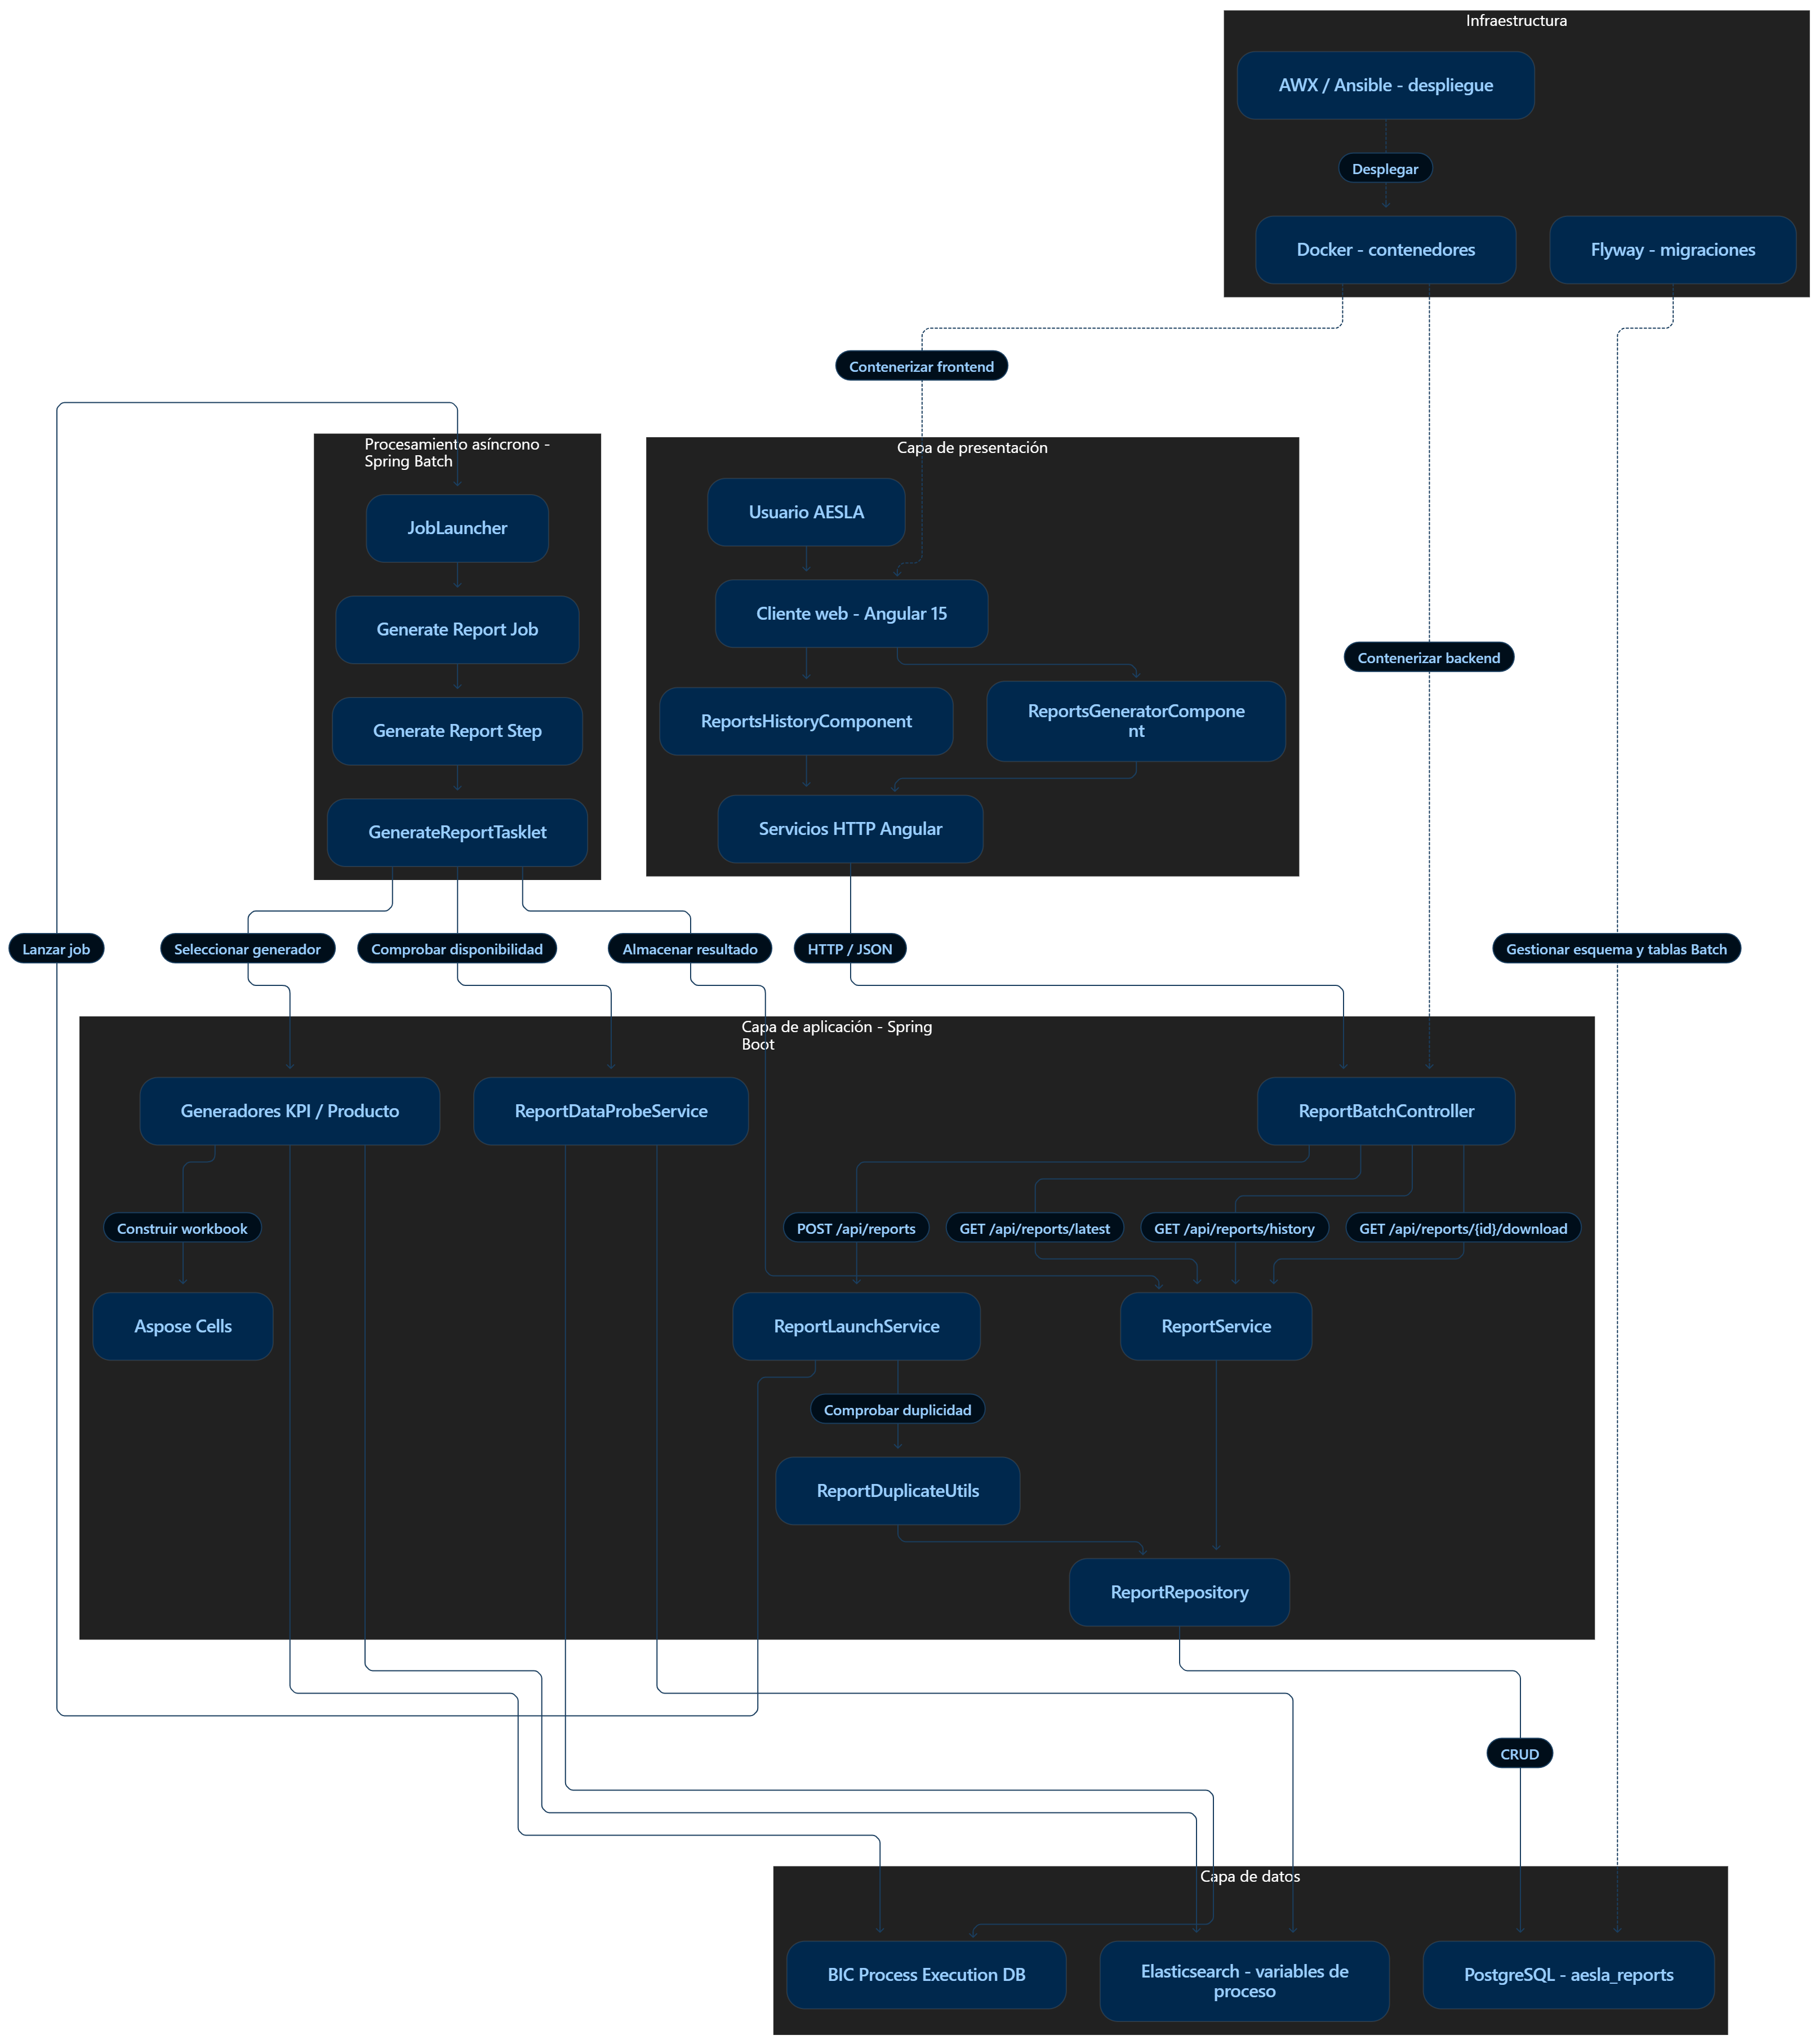
\includegraphics[width=\textwidth]{img/arquitectura_detallada.png}
  \caption{Arquitectura detallada del Report Service. Fuente: elaboración propia.}
  \label{fig:arquitectura-detallada}
\end{figure}

En la capa de presentación, el usuario interactúa con los componentes Angular
de generación e historial, que centralizan sus comunicaciones con el backend
a través de servicios HTTP. El punto de entrada en la capa de aplicación es
\texttt{ReportBatchController}, encargado de exponer las operaciones REST
utilizadas por el cliente.

Para una nueva generación, el controlador delega en
\texttt{ReportLaunchService}, que realiza la comprobación previa de
duplicidad antes de iniciar el job de Spring Batch. El procesamiento
asíncrono se articula mediante \texttt{JobLauncher}, un job, un step y
\texttt{GenerateReportTasklet}. Durante su ejecución se comprueba la
disponibilidad de datos mediante \texttt{ReportDataProbeService} y se
selecciona la lógica de generación correspondiente al tipo y categoría de
informe.

Los datos utilizados proceden de BIC Process Execution y Elasticsearch,
mientras que Aspose Cells proporciona las operaciones necesarias para la
construcción de los libros Excel. Finalmente, \texttt{ReportService}
centraliza el almacenamiento del resultado y utiliza
\texttt{ReportRepository} para persistir el contenido y sus metadatos en el
esquema \texttt{aesla\_reports} de PostgreSQL.

La infraestructura complementaria incluye Flyway para gestionar las
migraciones de base de datos, Docker para la contenerización de los servicios
y AWX/Ansible para automatizar su despliegue en los diferentes entornos.


%%%%%%%%%%%%%%%%%%%%%%%%%%%%%%%%%%%%%%%%%
% Evidencias de calidad de código       %
%%%%%%%%%%%%%%%%%%%%%%%%%%%%%%%%%%%%%%%%%

\section{Evidencias de calidad de código}
\label{ap:evidencias-sonar}

Las siguientes figuras recogen las capturas de SonarCloud utilizadas como
evidencia de las métricas de cobertura y duplicación presentadas en el
capítulo~6. En el cuerpo principal de la memoria se muestran únicamente los
valores iniciales y finales, mientras que las capturas completas se trasladan
a este apéndice para facilitar su consulta sin sobrecargar el capítulo de
implementación y pruebas.

\begin{figure}[H]
  \centering
  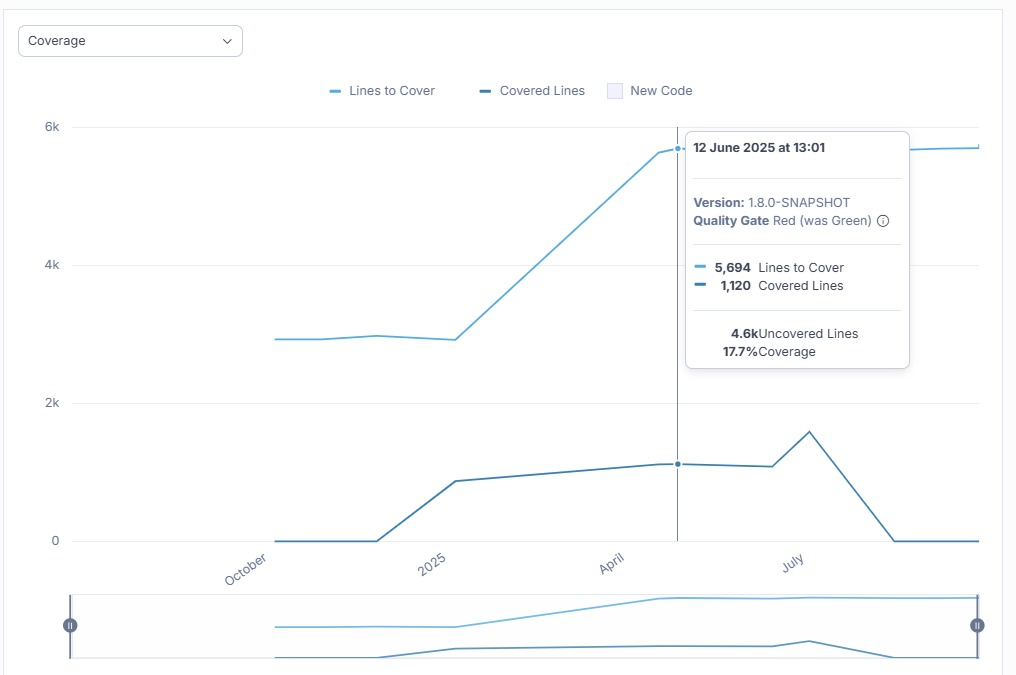
\includegraphics[width=0.85\textwidth]{img/coverage_before.jpeg}
  \caption{Captura de SonarCloud correspondiente a la cobertura inicial del proyecto: 17.7\%.}
  \label{fig:coverage-before}
\end{figure}

\begin{figure}[H]
  \centering
  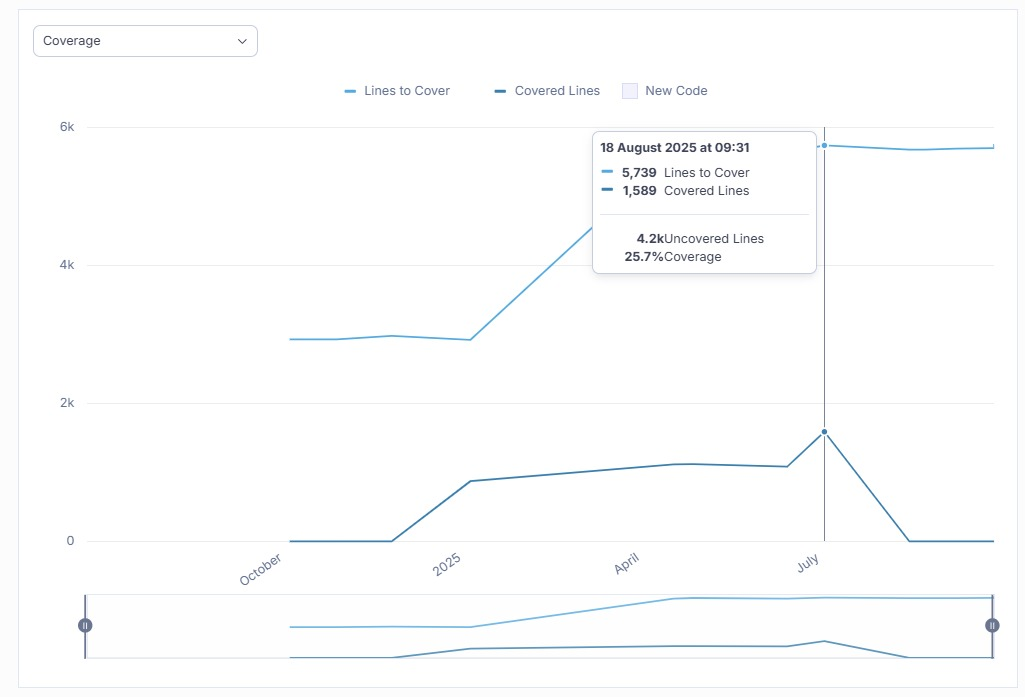
\includegraphics[width=0.85\textwidth]{img/coverage_after.jpeg}
  \caption{Captura de SonarCloud correspondiente a la cobertura final del proyecto: 25.7\%.}
  \label{fig:coverage-after}
\end{figure}

\begin{figure}[H]
  \centering
  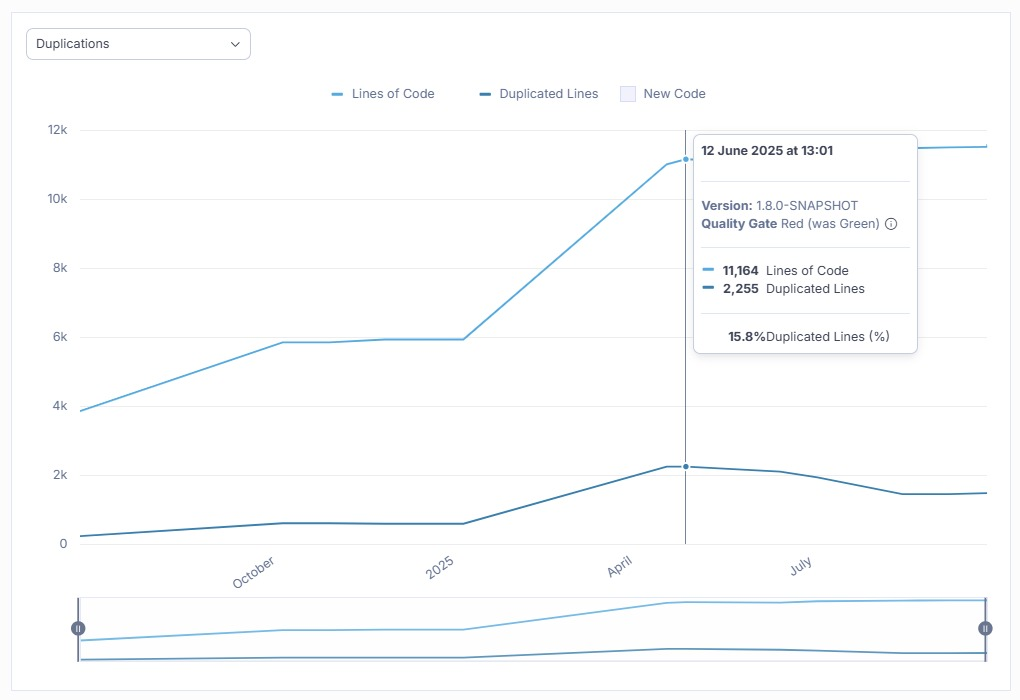
\includegraphics[width=0.85\textwidth]{img/duplications_before.jpeg}
  \caption{Captura de SonarCloud correspondiente a la duplicación inicial del proyecto: 15.8\%.}
  \label{fig:duplications-before}
\end{figure}

\begin{figure}[H]
  \centering
  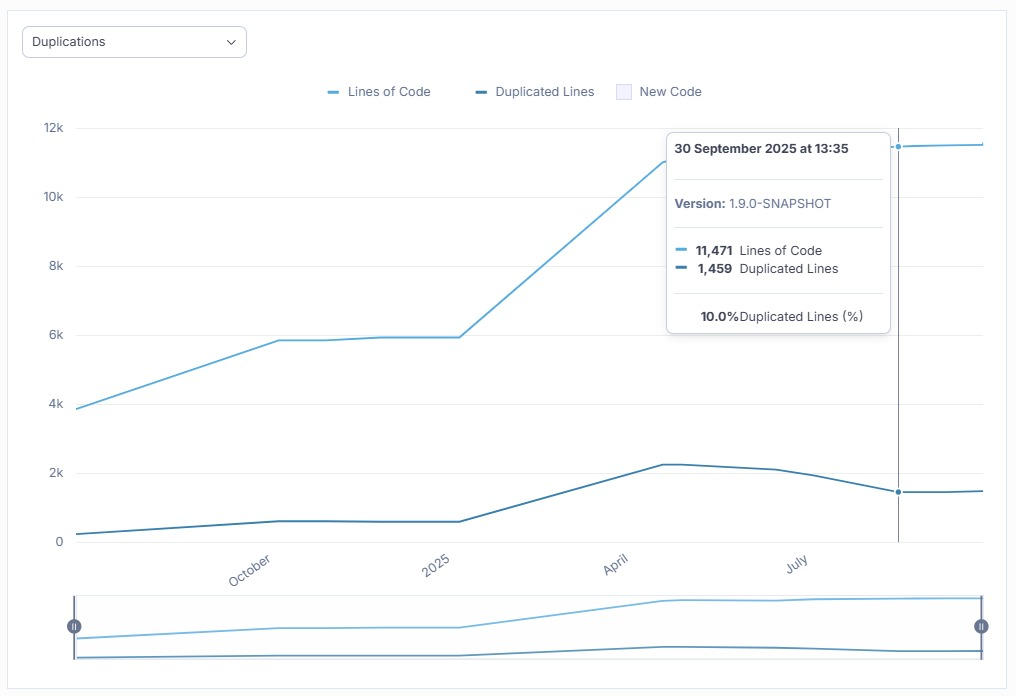
\includegraphics[width=0.85\textwidth]{img/duplications_after.jpeg}
  \caption{Captura de SonarCloud correspondiente a la duplicación final del proyecto: 10.0\%.}
  \label{fig:duplications-after}
\end{figure}